\mysection{Service Curves}\label{serviceCurves}

Resource models provide information about the processing capacities of the resources that are available within a system.
Thus, they characterize the service that can be provided by the system~\cite{mar}.
For every resource, whether communicational or computational, an own resource model has to be constructed.

\mysubsection{Resource Bounds}

We define the differential service function \(C[s, t)\) as the total number of available resource units, e.g. processor cycles or transmittable bits on a bus, within the time interval \([s, t): s,t \in \mathbb{R}\)~\cite{cho:08}.
While C models one concrete availability of a resource, in the framework of RTC we usually characterize a resource by its service curves~\cite{cho:08}:
\[\beta(\Delta t) = [\beta^{\, u}(\Delta t), \beta^{\, l}(\Delta t)]\]
The bounds are related by \[\forall t \leq s \leq 0: \beta^{l}(t-s) \leq C[s, t) \leq \beta^{u}(t-s)\]
meaning that all possible processing capacities of this component are located between the lower service curve \(\beta^{\, l}(\Delta t)\) and the upper service curve \(\beta^{\, u}(\Delta t)\).
Therefore, these curves set guaranteed lower and upper bounds on the processing units available at this resource over any time interval of length \(\Delta t\)~\cite{moy}.
In an analogue way to \(\overline{\alpha}(\Delta t)\) we can also define \(\overline{\beta}(\Delta t)\) as
\[[\overline{\beta}^{\, u}(\Delta t), \overline{\beta}^{\, l}(\Delta t)] = [(\gamma^{l})^{-1}(\beta^{\, u}), (\gamma^{u})^{-1}(\beta^{\, l})]\]
\(\overline{\beta}(\Delta t)\) directly depends on the number of events that can be processed per \(\Delta t\), yet it only has very few use cases.

\mysubsection{Handling Different Resource Availability Patterns}

The capacities of various resources, such as resources with full availability, but also with fluctuating service capacities, can be efficiently abstracted into curves~\cite{mar}.
When dealing with a simple unloaded processor with full availability, the service curve can be modeled by the linear function
\[\beta^{\, u}(\Delta t) = \beta^{\, l}(\Delta t) = APC \cdot \Delta t\] with \textbf{APC} being the constant number of available processing cycles per time interval (see \autoref{fig:simple_cpu})~\cite{mar}.

\begin{figure}
    \centering
    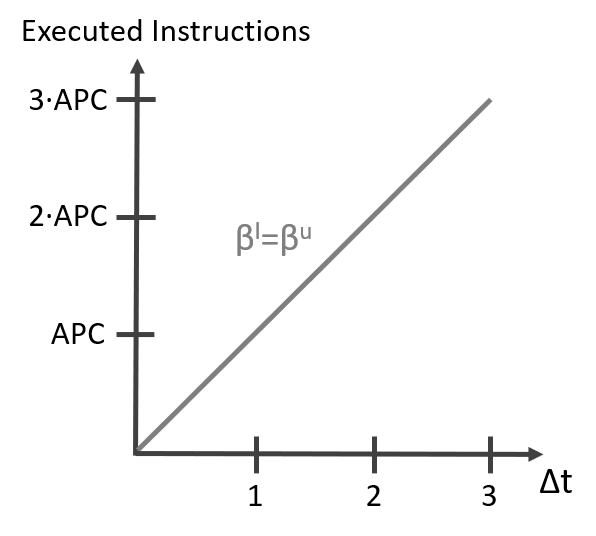
\includegraphics[width=0.6\columnwidth]{graphics/simple_cpu.png}
    \caption{Service curve of a simple CPU with full availability}\label{fig:simple_cpu}
\end{figure}

A popular example for resources with fluctuating availability are time division multiple access (\textbf{TDMA}) busses.
When communicating via a TDMA bus, information can be transmitted with a period \textbf{p} for \textbf{s} time units using the full bus bandwidth \textbf{b}.
Afterwards there is a waiting period of \(p-s\) time units until the bus gets allocated again (see \autoref{fig:tdma_bus})~\cite{mar}.

\begin{figure}
    \centering
    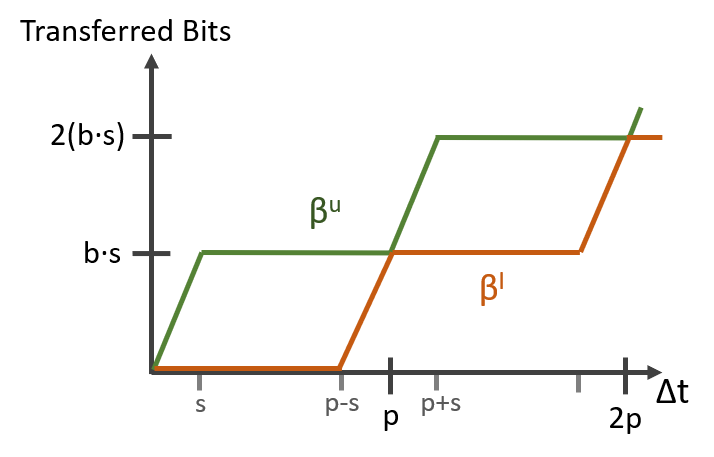
\includegraphics[width=0.8\columnwidth]{graphics/tdma_bus.png}
    \caption{Service curve of a simple TDMA bus}\label{fig:tdma_bus}
\end{figure}

\mysubsection{Service Curves of the Sample System}

Here we choose to use fully available CPUs as computational resources, with 4 or 5 million executable instructions per second (\textbf{MIPS}),
Additionally we use a TDMA bus as a communicational resource.
The available service of the bus is given by the bandwidth of 20 kilobits of transferrable information per second (\textbf{kbps}), a period of 10 and a slot length of 8.
The service curves of these resources are given by \autoref{fig:b-ins}.

\begin{figure}
    \centering
    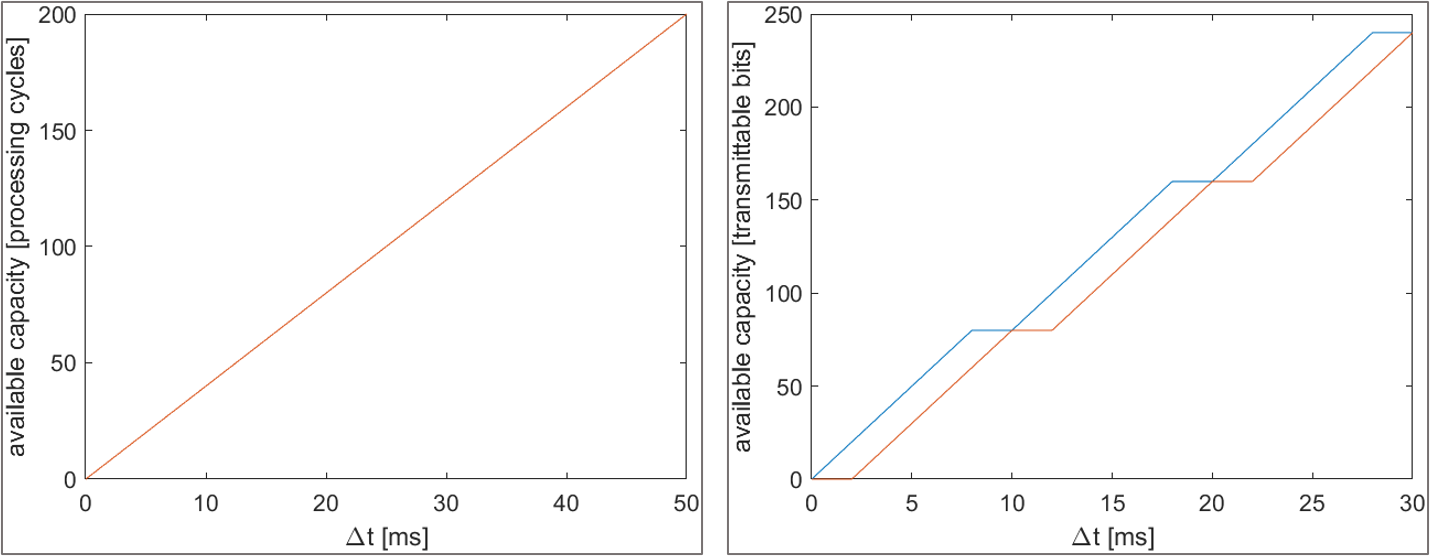
\includegraphics[width=\columnwidth]{graphics/example_b_ins.png}
    \caption{Service curves of the sample system's 4 MIPS CPU (left) and it's TDMA bus (right)}\label{fig:b-ins}
\end{figure}